\documentclass{article}
\usepackage[utf8]{inputenc}
\usepackage{graphicx}
\usepackage{subfig}
\usepackage{amsmath}
\newpage
\newpage
\title{Digital Logic Design Assignment 10 - EC2019-39}
\author{Chetan sarigala }
\date{December 16, 2020}
\begin{document}
\maketitle
\begin{document}
\section{EC2019 39 }

  

         \begin{question}
       The state transition diagram for the circuit is
\begin{figure}[!ht]
\centerline{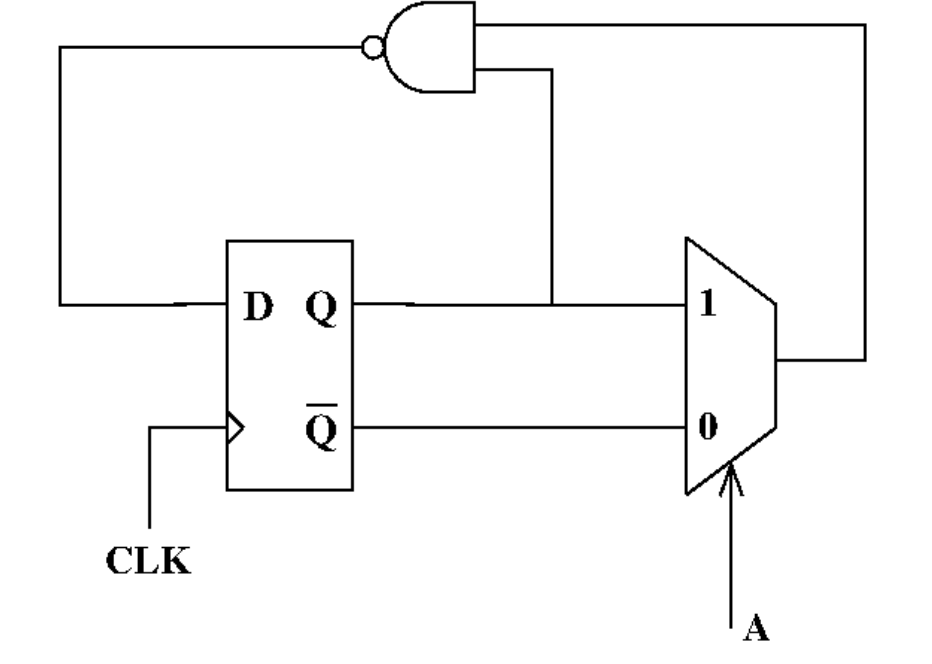
\includegraphics[scale=1]{fig1.PNG}}
	\caption{}
	\label{fig1.PNG}
\end{figure}

\begin{figure}[!ht]
\centerline{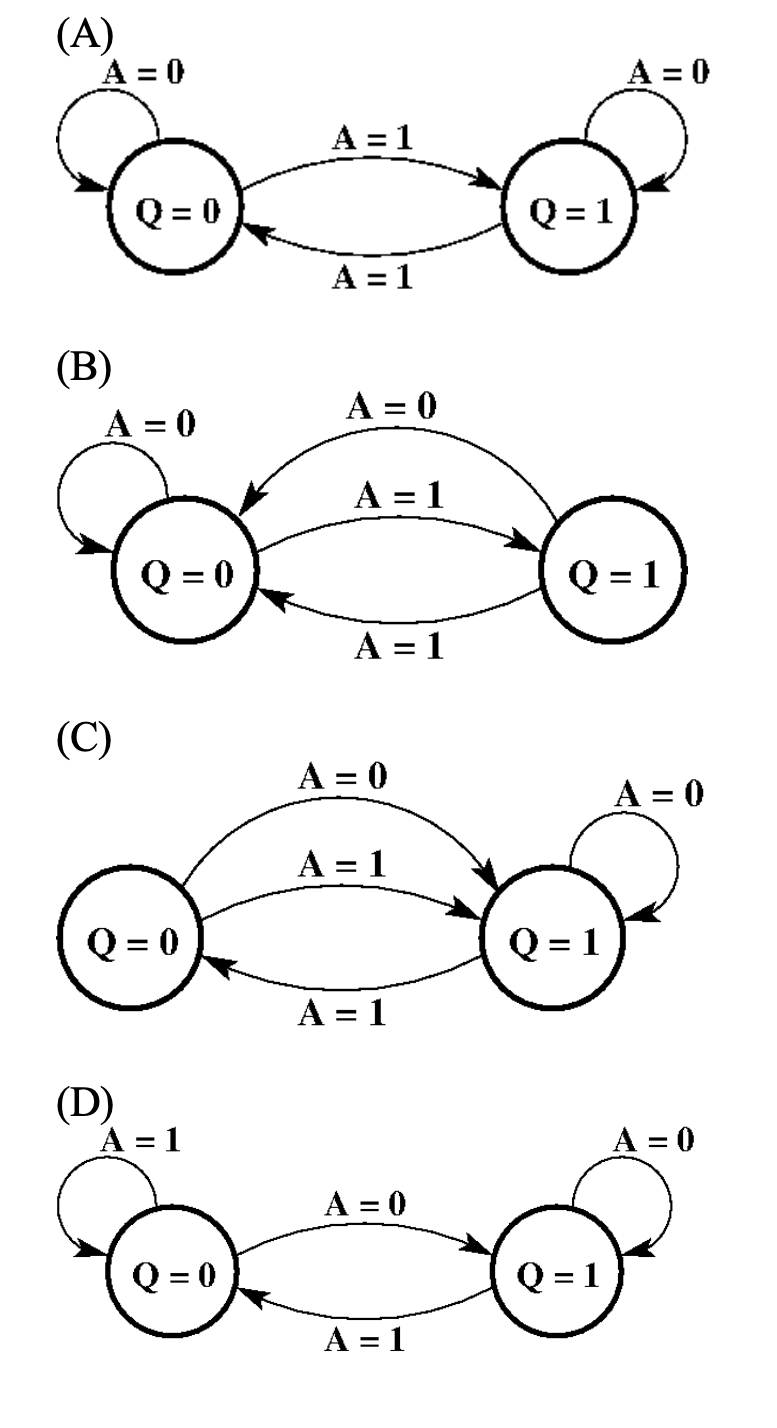
\includegraphics[scale=.5]{fig2.PNG}}
	\caption{}
	\label{fig2.PNG}
\end{figure}
 \end{question}
\begin{answer}



\title{ANSWER}.


The follwing circuit (figure 1) has one D flip flop, one 2*1 multiplexer and one nand gate.

Now let us assume that output of the multiplexer as y.

if A=0 then the output y=1.

D = \overline{Q.y}.

 D = \overline{Q}+\overline{y}.
  
the possible ways for output Q=0,1.

now let us assume that the output Q = 0 then \overline{Q}=1.

then D = 1 + 0 .
     D = 1.
     
     when A = 1
     
     then the output y = 0.
     
     then D = \overline{Q.y}.
     
     D = 1.
     
Now let us take Q = 1.

then when A = 0 , y = 1.

D = \overline{Q}+\overline{y}

D = 0

Similarly,

if A = 1, y = 0.

then D = \overline{Q.y}

D = 0 + 1.

D = 1.

 Therfore option (C) is correct.
  

 \begin{figure}[!ht]
\centerline{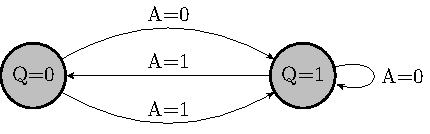
\includegraphics[scale=2]{10.pdf}}
	
	\label{10.pdf}
\end{figure}

 \begin{figure}[!ht]
\centerline{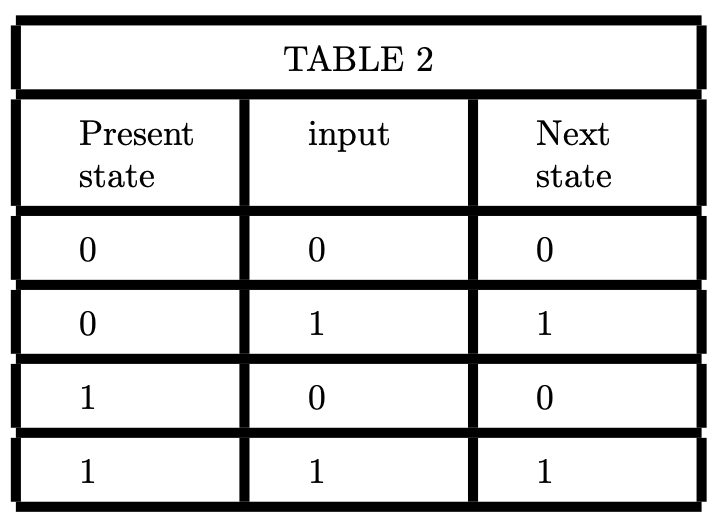
\includegraphics[scale=2]{state.png}}
	
	\label{state.png}
\end{figure}
\end{answer}


        

      

      



  

\end{document}



